\providecommand\ExamFontPath{../../../字体/}
\documentclass[fontset=exam]{exam-zh}
\usepackage{longtable,booktabs,array,calc,multirow,fvextra}
\usepackage[normalem]{ulem}
\providecommand{\hl}[1]{#1}
\providecommand{\ul}[1]{\uline{#1}}
\DefineVerbatimEnvironment{verbatim}{Verbatim}{breaklines=true,fontsize=\small}
\providecommand{\tightlist}{\setlength{\itemsep}{0pt}\setlength{\parskip}{0pt}}
\newcommand{\pandocbounded}[1]{#1}
\setlength{\emergencystretch}{3em}
\setlength{\tabcolsep}{2pt}
\examsetup{page/size=a4paper}
\title{厦门大学 2014—2015 年 期中考试}
\subject[4em]{热学}
\begin{document}
\maketitle
\fancyfoot[C]{第 \thepage 页（共 \pageref*{LastPage} 页）}
1．（18 分）

一打气筒，每打一次气可将原来压强为\(p_{0} = 1.0\text{a}\text{t}\text{m}\)，温度为\(t_{0} = 27.0^{0}\text{C}\)，体积\(V_{0} = 4.0\text{L}\)的空气压缩到容器内。设容器的体积\(V = 1.5 \times 10^{3}\text{L}\)，打气之前容器内空气的压强和温度分别为\(p_{0}\)和\(t_{0}\)。设空气可视为理想气体，问要大打几次气才能使容器内空气的温度为\(t = 45^{0}\text{C}\)，压强为\(p = 2.0\text{a}\text{t}\text{m}\)？

2. （18 分）

一定量的理想气体，初态体积为\emph{V}\textsubscript{0}，压强为\emph{p}\textsubscript{0}。先对气体等压加热，使体积膨胀为 2\emph{V}\textsubscript{0}，然后等容加热，使压强增大为 2\emph{p}\textsubscript{0} ，最后通过绝热过程使体积膨胀到 16 \emph{V}\textsubscript{0}。已知气体的定压摩尔热容\(C_{p,m} = \frac{5}{2}R\)（\emph{R}为气体普适常量），求

（1）全过程中内能的变化；

（2）全过程中气体吸收的热量和对外所做的功。

3. （18 分）

一根长为 76cm 的玻璃管，上端封闭，下端插入水银中，水银充满管子的一部分，管子另一部分封闭有 0.1mol 的空气，设外界压强保持在 76cmHg，空气的定容摩尔取\(C_{V} = \frac{5}{2}R\)。若管内空气的温度降低 10\textsuperscript{0}C，求：\par\medskip{\centering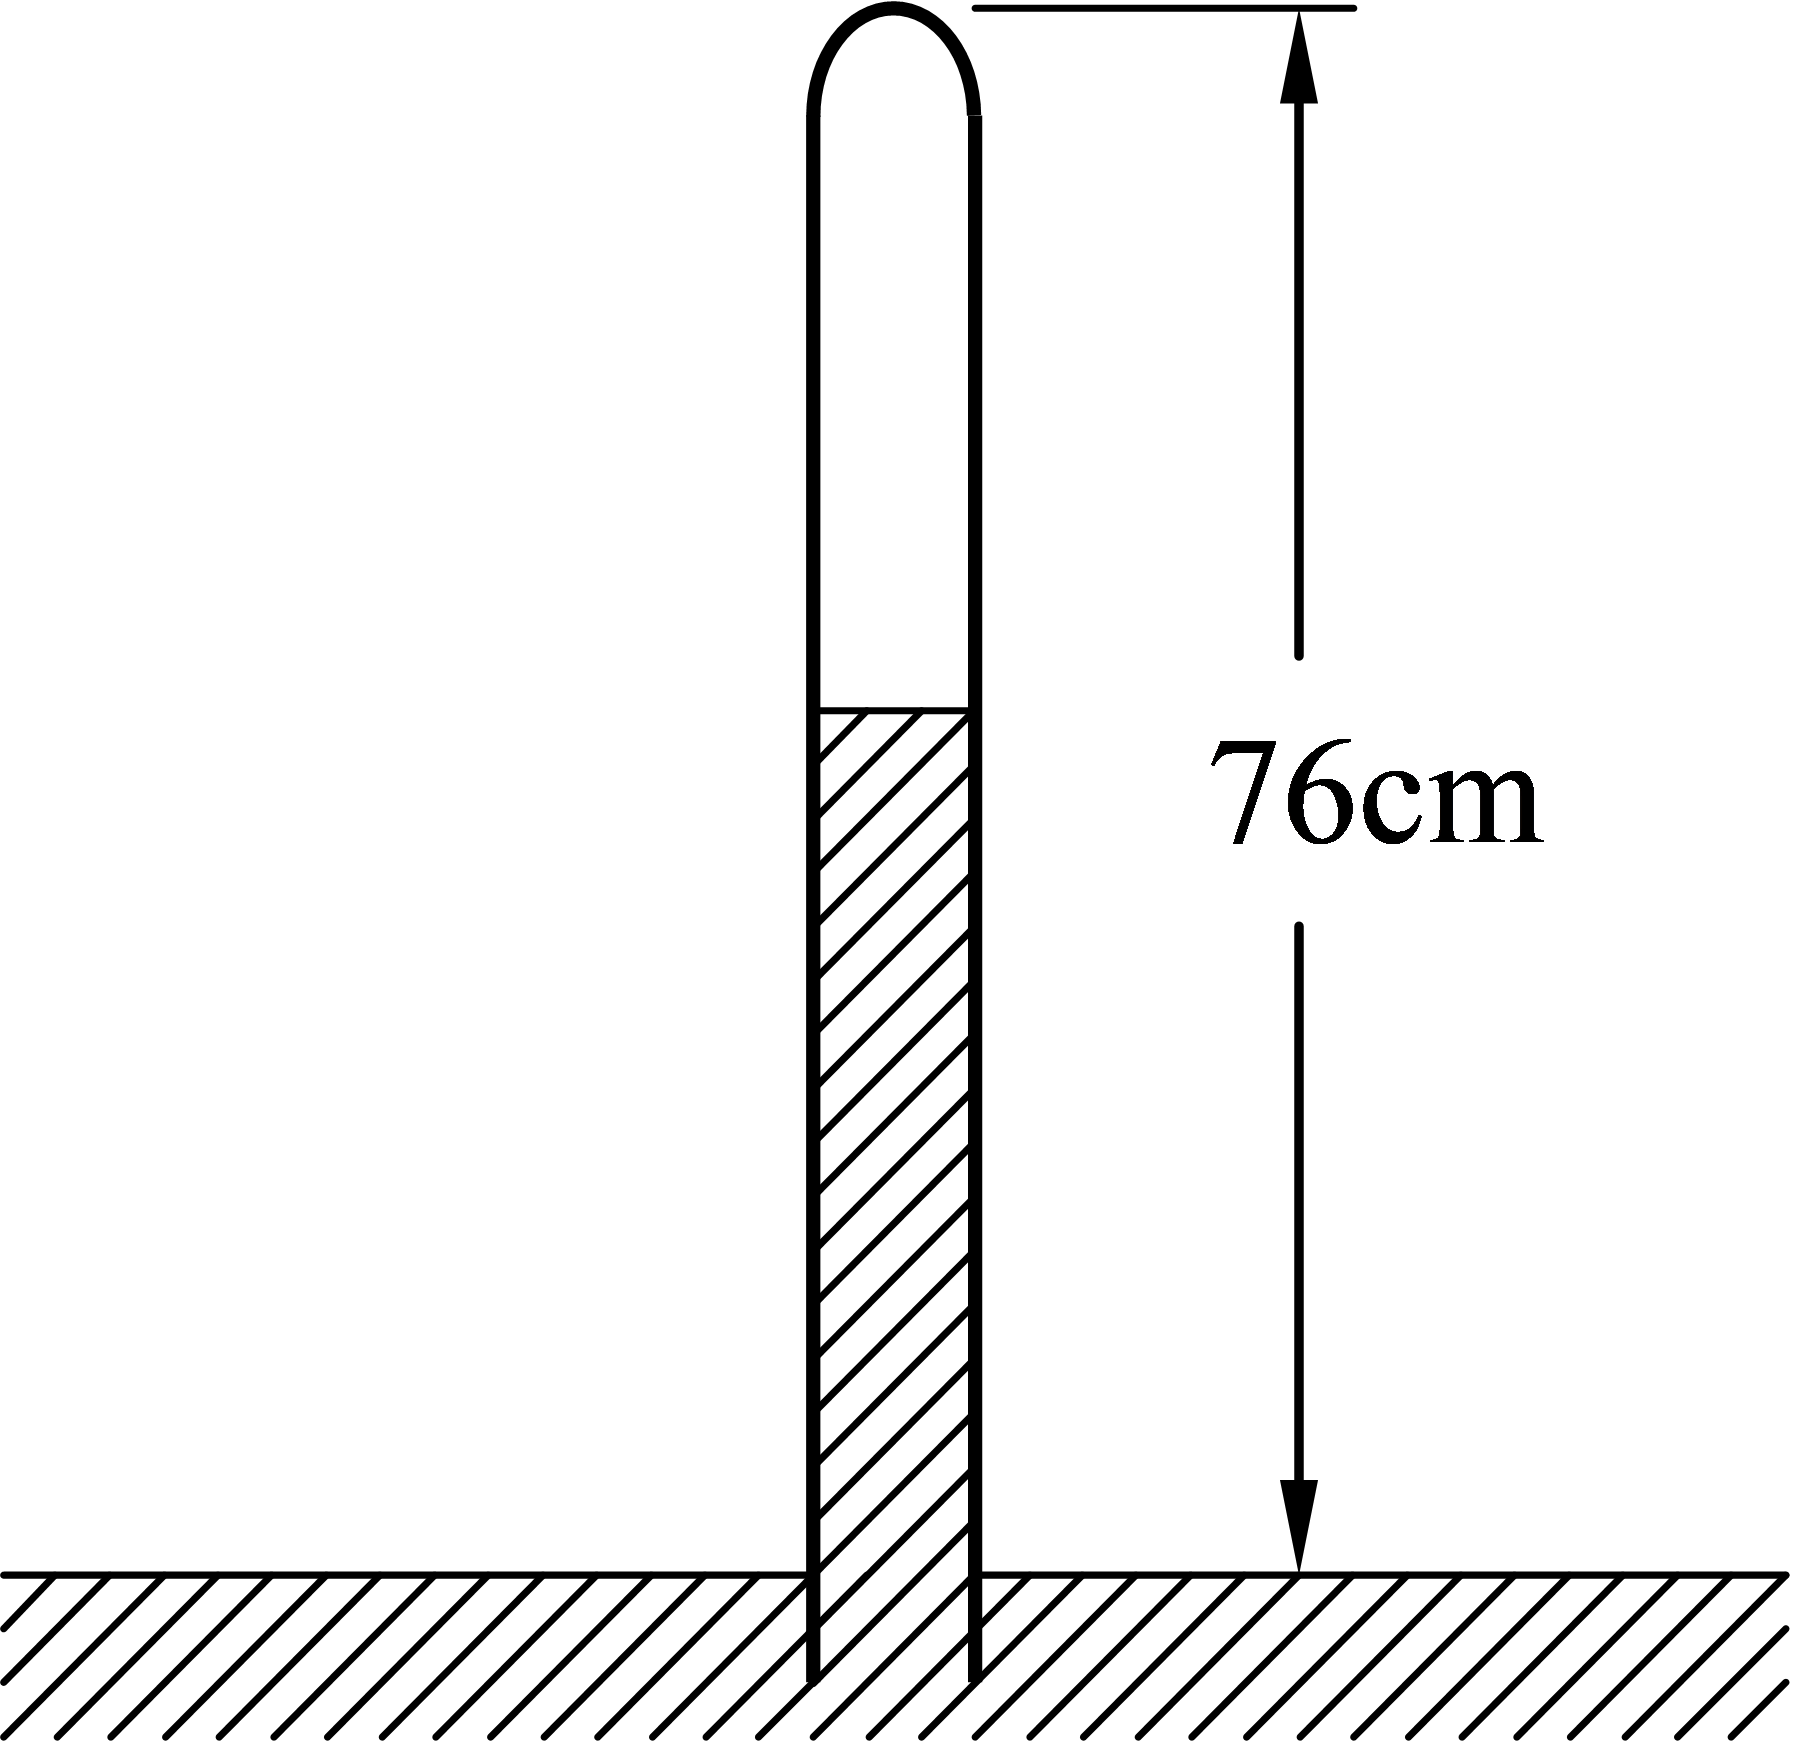
\includegraphics[width=5cm,height=4cm,keepaspectratio]{figures/image29.png}\par}\medskip

（1）管内空气内能的改变，是增大还是减小？

（2）管内空气对外所做的功，是正功还是负功？

（3）管内空气与外界交换的热量，是吸热还是放热？

4.（16 分）\par\medskip{\centering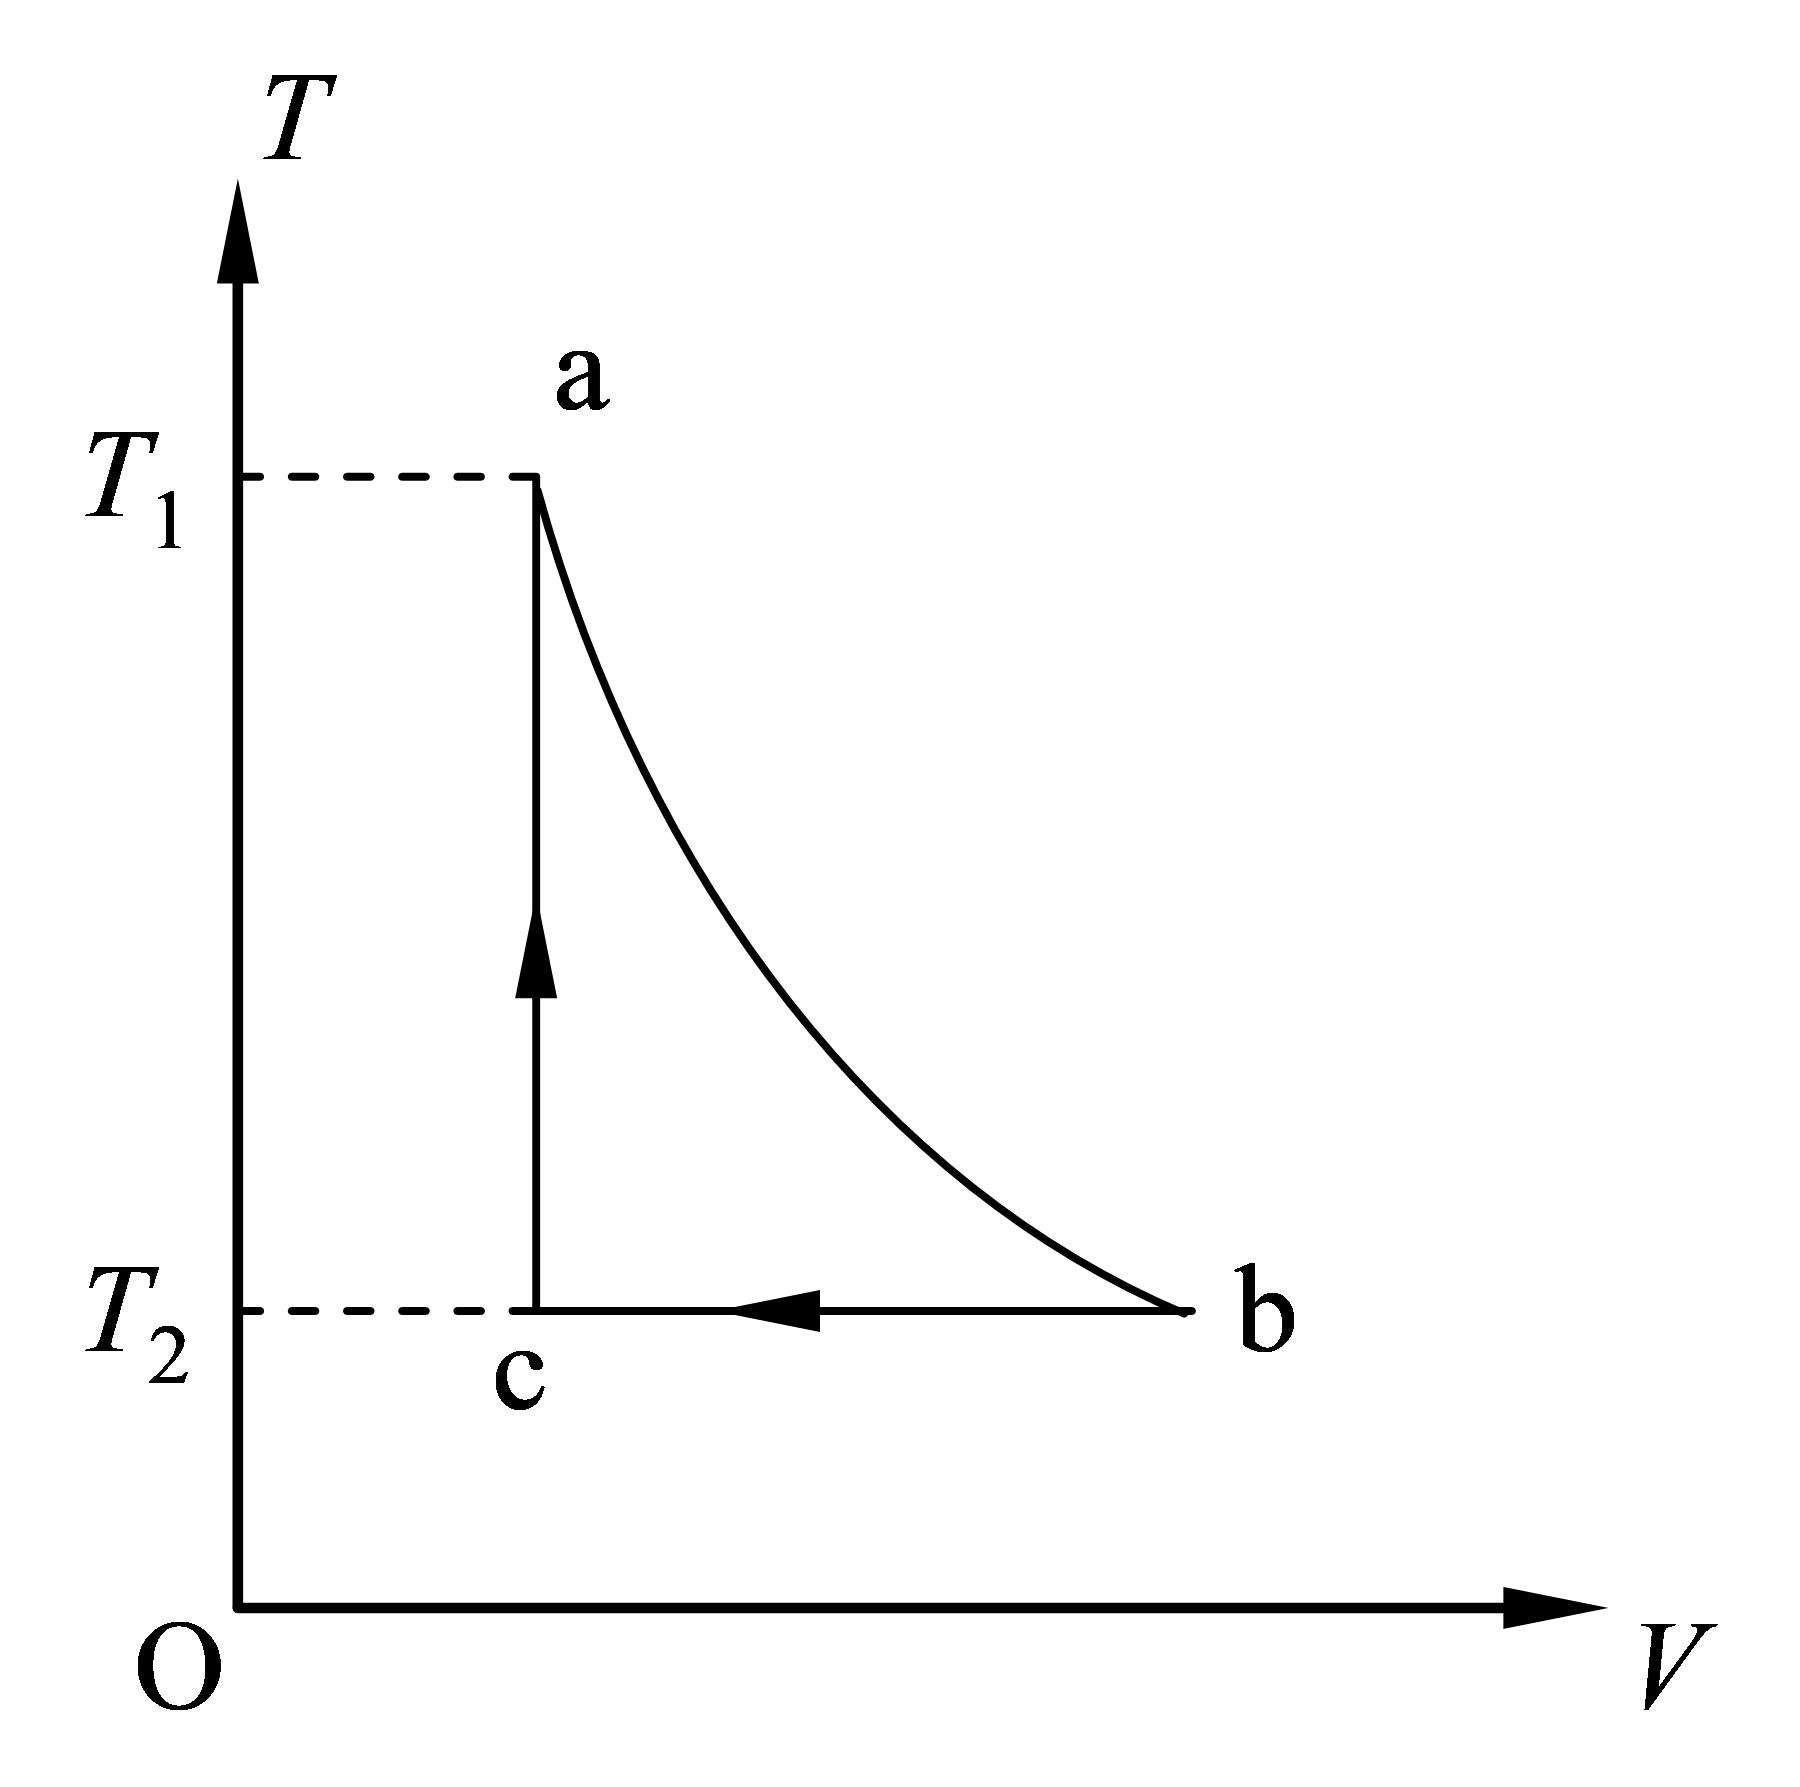
\includegraphics[width=5cm,height=4cm,keepaspectratio]{figures/image35.png}\par}\medskip

某热机的循环过程如图所示，其中 ab 为绝热过程，bc 为等温过程，ca 为等容过程。设工作物质为理想气体，证明热机的效率为

\[\eta = 1 - \frac{ln\beta}{\beta - 1}\]

式中\(\beta = T_{1}/T_{2}\)。

5．（15 分）

在温度分别为 227°C 和 27°C 的恒温热源之间工作的热机，在一个循环中从高温热源吸收的热量为 300J。

（1）假设该热机在一个循环中对外所做净功为 100J，则此热机是否为可逆热机，为什么？

（2）假设该热机为可逆热机，则在一个循环中对外所做净功为多少？

（3）假设该热机为可逆热机，今使其逆向运转，则为使在一个循环中工作物质从低温热源吸收 60J 的热量，外界对系统所做的净功是多少？

6.（15 分）

1mol 的理想气体分别经以下三个准静态过程使体积膨胀为原来的两倍：

（1）等压过程

（2）等温过程

（3）绝热过程

试分别求出上述三个过程中气体的熵变。设气体的定容摩尔热容\(C_{V,m} = \frac{3}{2}R\)（\emph{R}为气体普适常量）。

\end{document}
